\documentclass[aspectratio=169,11pt]{beamer}

% ============================================================
% PACKAGES
% ============================================================

\usepackage{graphicx}
\usepackage{tikz}
\usetikzlibrary{
    positioning,
    arrows.meta,
    shapes.geometric,
    fit,
    backgrounds
}
\usepackage{xcolor}
\usepackage{booktabs}
\usepackage{tabularx}
\usepackage{array}
\usepackage{ragged2e}
\usepackage{hyperref}

% ============================================================
% COLOURS
% ============================================================

\definecolor{GEUBlue}{RGB}{20,55,105}
\definecolor{GEULightBlue}{RGB}{238,244,251}
\definecolor{GEUGrey}{RGB}{90,90,90}
\definecolor{GEULightGrey}{RGB}{245,246,248}
\definecolor{DarkGrey}{RGB}{55,55,55}

% ============================================================
% THEME & GEOMETRY ADJUSTMENTS
% ============================================================

\usetheme{default}

\setbeamertemplate{navigation symbols}{}
\setbeamertemplate{blocks}[rounded][shadow=false]

\setbeamercolor{normal text}{fg=black,bg=white}
\setbeamercolor{frametitle}{fg=GEUBlue}
\setbeamercolor{structure}{fg=GEUBlue}
\setbeamercolor{block title}{fg=GEUBlue,bg=GEULightBlue}
\setbeamercolor{block body}{fg=black,bg=GEULightBlue}

\setbeamerfont{frametitle}{size=\Large,series=\bfseries}

\setbeamersize{text margin left=0.6cm, text margin right=0.6cm}

% ============================================================
% LOGO
% ============================================================

\newcommand{\GEULogo}{graphicera_logo.png}

% ============================================================
% HEADER
% ============================================================

\setbeamertemplate{headline}{%
  \begin{tikzpicture}[remember picture,overlay]
    \node[
        anchor=north east,
        xshift=-0.30cm,
        yshift=-0.12cm
    ]
    at (current page.north east)
    {\IfFileExists{\GEULogo}{\includegraphics[height=0.55cm]{\GEULogo}}{\rule{0.55cm}{0.55cm}}};
  \end{tikzpicture}%
  \vspace{0.45cm}
}

% ============================================================
% FRAME TITLE
% ============================================================

\setbeamertemplate{frametitle}{%
  \vspace{-0.2cm}%
  \insertframetitle\par
  \vspace{0.02cm}%
  \textcolor{GEUBlue}{\rule{\textwidth}{0.8pt}}%
  \vspace{0.1cm}%
}

% ============================================================
% FOOTER
% ============================================================

\setbeamertemplate{footline}{%
  \leavevmode
  \hbox{%
  \begin{beamercolorbox}[
      wd=.82\paperwidth,
      ht=0.28cm,
      dp=0.08cm,
      leftskip=.3cm
  ]{author in head/foot}
    \tiny
    Department of Computer Science \& Engineering |
    Graphic Era (Deemed to be University)
  \end{beamercolorbox}%
  \begin{beamercolorbox}[
      wd=.18\paperwidth,
      ht=0.28cm,
      dp=0.08cm,
      rightskip=.3cm
  ]{date in head/foot}
    \hfill\tiny\insertframenumber/\inserttotalframenumber
  \end{beamercolorbox}}
}

% ============================================================
% HELPER COMMANDS
% ============================================================

\newcommand{\smallnote}[1]{%
    \vspace{0.05cm}%
    {\tiny\color{GEUGrey}#1}%
}

\newcommand{\tagbox}[1]{%
    \colorbox{GEULightBlue}{%
        \textcolor{GEUBlue}{\scriptsize\textbf{#1}}%
    }%
}

% ============================================================
% TITLE INFORMATION
% ============================================================

\title{
    \textbf{Project-Based Learning}\\[2mm]
    \large Phase-I Evaluation
}

\author{
    \textbf{NEXUS}\\
    AI-Powered Distributed Data Processing
    \& Compute Orchestration Platform\\
    Team ID: OS-DBMS-V-2026-T099
}

\institute{
    Department of Computer Science \& Engineering\\
    Graphic Era (Deemed to be University), Dehradun
}

\date{Academic Session 2026--27}

% ============================================================
% DOCUMENT
% ============================================================

\begin{document}

% ============================================================
% 1. TITLE SLIDE
% ============================================================

\begin{frame}[plain]

\begin{tikzpicture}[remember picture,overlay]

\draw[
    GEUBlue,
    line width=3pt
]
(current page.north west)
--
(current page.north east);

\node[
    anchor=north east,
    xshift=-0.45cm,
    yshift=-0.35cm
]
at (current page.north east)
{\IfFileExists{\GEULogo}{\includegraphics[height=0.9cm]{\GEULogo}}{\rule{0.9cm}{0.9cm}}};

\node[
    align=center,
    text width=.88\paperwidth
]
at ([yshift=.15cm]current page.center)
{

{\color{GEUBlue}
\fontsize{22}{26}\selectfont
\bfseries PROJECT-BASED LEARNING}

\\[2mm]

{\fontsize{16}{20}\selectfont
PHASE-I EVALUATION}

\\[5mm]

{\color{GEUBlue}
\fontsize{20}{24}\selectfont
\bfseries NEXUS}

\\[1.5mm]

{\color{GEUGrey}
\normalsize
AI-Powered Distributed Data Processing\\
\& Compute Orchestration Platform}

\\[4mm]

{\color{GEUBlue}
\small
Team ID: OS-DBMS-V-2026-T099}

};

\node[
    align=center,
    anchor=south,
    yshift=.35cm
]
at (current page.south)
{
\small\bfseries
Department of Computer Science \& Engineering\\
Graphic Era (Deemed to be University), Dehradun\\[-0.5mm]
\tiny Academic Session 2026--27
};

\end{tikzpicture}

\end{frame}


% ============================================================
% 2. TEAM & MENTOR DETAILS
% ============================================================

\begin{frame}{Team \& Mentor Details}

\begin{columns}[T,totalwidth=\textwidth]

\column{.47\textwidth}

\begin{block}{Project Information}
\small
\begin{tabular}{@{}ll@{}}
\textbf{Team ID:} & OS-DBMS-V-2026-T099 \\[0.5mm]
\textbf{Team Name:} & Avengers \\[0.5mm]
\textbf{Semester:} & 5th \\[0.5mm]
\textbf{Domain:} & AI / DBMS / OS / Dist. Sys. \\[0.5mm]
\textbf{Project Type:} & Full-Stack Web Application
\end{tabular}
\end{block}

\vspace{0.0mm}

\begin{block}{Project Title}
\small
\textbf
 NEXUS: AI-Powered Distributed Data Processing \& Compute Orchestration Platform
\end{block}

\column{.50\textwidth}

\begin{block}{Team Members}
\small
\textbf{1. Team Lead}\\
Pareek, Raghvander -- 240211322\\[1.5mm]
\textbf{2. Team Member}\\
Kumar Singh, Tanishk -- 240211960\\[1.5mm]
\textbf{3. Team Member}\\
Kumar Singh, Tushar -- 240211961\\[1.5mm]
\textbf{4. Team Member}\\
Raj Kathait, Soyam -- 240211683
\end{block}

\end{columns}

\vspace{1.5mm}

\begin{block}{Mentor Details}
\small
\begin{tabular}{@{}p{0.68\textwidth} r@{}}
\textbf{Mentor:} Mr.Yogesh Lohumi & \textbf{Interactions:} 2
\end{tabular}
\end{block}

\end{frame}


% ============================================================
% 3. PROBLEM STATEMENT & MOTIVATION
% ============================================================

\begin{frame}{Problem Statement \& Motivation}

\begin{block}{Problem Statement}
\small
Modern organisations generate large amounts of data, but analysing this data can be difficult for users lacking SQL knowledge. Analytical queries require variable CPU, memory, and runtime. Traditional systems lack an integrated mechanism connecting \textbf{query understanding, optimisation, scheduling, and resource management}.

\textbf{NEXUS proposes a unified platform combining AI data interaction with DBMS, OS, and Distributed Systems principles.}
\end{block}

\vspace{1mm}

\begin{columns}[T,totalwidth=\textwidth]

\column{.48\textwidth}

\textbf{\color{GEUBlue}\small Why is this a problem?}
\begin{itemize}\itemsep1pt
\item[\tiny$\bullet$] \scriptsize Users need SQL knowledge for analysis.
\item[\tiny$\bullet$] \scriptsize Complex queries consume heavy resources.
\item[\tiny$\bullet$] \scriptsize Jobs have varying execution requirements.
\item[\tiny$\bullet$] \scriptsize Query \& resource management are siloed.
\end{itemize}

\column{.48\textwidth}

\textbf{\color{GEUBlue}\small NEXUS Approach}
\begin{itemize}\itemsep1pt
\item[\tiny$\bullet$] \scriptsize Natural-language interface for queries.
\item[\tiny$\bullet$] \scriptsize AI converts user queries to SQL.
\item[\tiny$\bullet$] \scriptsize SQL is validated, optimized \& scheduled.
\item[\tiny$\bullet$] \scriptsize Concurrent execution with visual output.
\end{itemize}

\end{columns}

\end{frame}


% ============================================================
% 4. STATE OF THE ART
% ============================================================

\begin{frame}{State of the Art \& Research Gap}

\begin{columns}[T,totalwidth=\textwidth]

\column{.48\textwidth}

\textbf{\color{GEUBlue}\small Existing Solutions}
\begin{itemize}\itemsep1pt
\item[\tiny$\bullet$] \scriptsize Database Management Systems / SQL Clients
\item[\tiny$\bullet$] \scriptsize BI Dashboards \& Data-analysis software
\item[\tiny$\bullet$] \scriptsize AI Natural Language-to-SQL tools
\item[\tiny$\bullet$] \scriptsize Distributed data-processing platforms
\end{itemize}

\vspace{1mm}

\textbf{\color{GEUBlue}\small Identified Gap}
\scriptsize
AI tools focus heavily on NL-to-SQL generation without execution management. Distributed execution systems target experienced developers.

\column{.48\textwidth}

\textbf{\color{GEUBlue}\small NEXUS Research Direction}

\begin{center}
\tagbox{AI Query Understanding}

\vspace{1mm}
$\downarrow$
\vspace{1mm}

\tagbox{SQL Validation + Optimisation}

\vspace{1mm}
$\downarrow$
\vspace{1mm}

\tagbox{OS-Inspired Job Scheduling}

\vspace{1mm}
$\downarrow$
\vspace{1mm}

\tagbox{Distributed Worker Execution}
\end{center}

\end{columns}

\vfill
\smallnote{Contribution: Integration of NL-to-SQL, query optimisation, and OS scheduling into one platform.}

\end{frame}


% ============================================================
% 5. OBJECTIVES
% ============================================================

\begin{frame}{Objectives}

\textbf{\color{GEUBlue}\small Project Objectives}

\vspace{1mm}

\begin{columns}[T,totalwidth=\textwidth]
\column{.50\textwidth}
\begin{enumerate}\itemsep1pt
\scriptsize
\item Interactive web app for data analysis.
\item Upload and manage structured datasets.
\item Ask analytical queries in natural language.
\item Convert NL requests to SQL via LLMs.
\item Validate SQL for safety and correctness.
\item Optimise queries before execution.
\end{enumerate}

\column{.48\textwidth}

\begin{enumerate}\setcounter{enumi}{6}\itemsep1pt
\scriptsize
\item Implement job queue \& CPU scheduling.
\item Execute via multiple worker processes.
\item Monitor CPU, memory \& worker status.
\item Maintain execution logs and history.
\item Provide visual results \& AI explanations.
\end{enumerate}
\end{columns}

\vspace{3mm}

\begin{center}
\colorbox{GEULightBlue}{
\parbox{.90\textwidth}{
\centering\scriptsize
\textbf{Key Objective:} Transform natural-language analytical requests into validated, optimized, and scheduled computational jobs.
}}
\end{center}

\end{frame}


% ============================================================
% 6. PROJECT GOALS & MILESTONES
% ============================================================

\begin{frame}{Project Goals \& Milestones}

\begin{columns}[T,totalwidth=\textwidth]

\column{.48\textwidth}

\textbf{\color{GEUBlue}\small Major Project Goals}
\begin{itemize}\itemsep1.5pt
\item[\tiny$\bullet$] \scriptsize Role-based user authentication
\item[\tiny$\bullet$] \scriptsize Schema understanding \& upload engine
\item[\tiny$\bullet$] \scriptsize Natural-language query parsing
\item[\tiny$\bullet$] \scriptsize SQL safety validation \& query optimisation
\item[\tiny$\bullet$] \scriptsize Job queue, multi-worker execution \& monitoring
\end{itemize}

\column{.48\textwidth}

\textbf{\color{GEUBlue}\small Development Milestones}
\begin{enumerate}\itemsep1.5pt
\scriptsize
\item Requirement analysis \& architecture
\item PostgreSQL database implementation
\item Frontend user interface setup
\item AI NL-to-SQL integration
\item Scheduler \& worker engine
\item System testing \& performance evaluation
\end{enumerate}

\end{columns}

\vspace{4mm}

\begin{center}
\colorbox{GEULightBlue}{
\parbox{.88\textwidth}{
\centering\scriptsize
\textbf{Development Strategy:} Build and validate incrementally, verifying each architectural layer prior to complete system-level integration.
}}
\end{center}

\end{frame}


% ============================================================
% 7. PROPOSED SOLUTION
% ============================================================

\begin{frame}{Proposed Solution}

\begin{center}
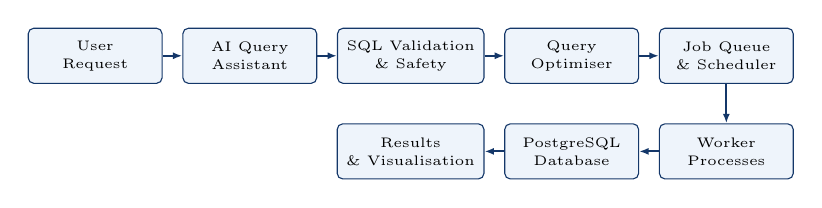
\begin{tikzpicture}[
node distance=2mm and 2.5mm,
box/.style={
    rectangle,
    rounded corners=2pt,
    draw=GEUBlue,
    fill=GEULightBlue,
    minimum width=1.7cm,
    minimum height=7mm,
    align=center,
    font=\fontsize{5.5}{6.5}\selectfont
},
arrow/.style={
    -{Latex[length=1.2mm]},
    thick,
    draw=GEUBlue
}
]

\node[box] (input) {User\\Request};
\node[box,right=of input] (ai) {AI Query\\Assistant};
\node[box,right=of ai] (validate) {SQL Validation\\\& Safety};
\node[box,right=of validate] (opt) {Query\\Optimiser};
\node[box,right=of opt] (job) {Job Queue\\\& Scheduler};

\node[box,below=5mm of job] (worker) {Worker\\Processes};
\node[box,left=of worker] (db) {PostgreSQL\\Database};
\node[box,left=of db] (result) {Results\\\& Visualisation};

\draw[arrow] (input) -- (ai);
\draw[arrow] (ai) -- (validate);
\draw[arrow] (validate) -- (opt);
\draw[arrow] (opt) -- (job);
\draw[arrow] (job) -- (worker);
\draw[arrow] (worker) -- (db);
\draw[arrow] (db) -- (result);

\end{tikzpicture}
\end{center}

\vspace{1mm}

\begin{columns}[T,totalwidth=\textwidth]

\column{.48\textwidth}
\textbf{\color{GEUBlue}\small User Workflow}
\begin{enumerate}\itemsep1pt
\scriptsize
\item Upload/select target dataset
\item Ask query in natural language
\item System validates \& optimises generated SQL
\item Job queued, scheduled, and executed
\item View visual results \& explanations
\end{enumerate}

\column{.48\textwidth}
\textbf{\color{GEUBlue}\small Operational Flow}
\begin{block}{Execution Pipeline}
\scriptsize
\textbf{Prompt:} ``Find top ten cities by revenue'' $\rightarrow$
AI Conversion $\rightarrow$ Safety Check $\rightarrow$ Optimiser $\rightarrow$ OS Scheduler $\rightarrow$ Multi-Worker Execution $\rightarrow$ Result Display
\end{block}

\end{columns}

\end{frame}


% ============================================================
% 8. SYSTEM ARCHITECTURE (FIXED OVERLAP)
% ============================================================

\begin{frame}{System Architecture}

\begin{center}
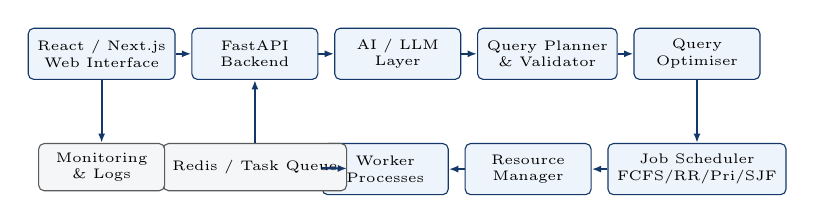
\begin{tikzpicture}[
node distance=2mm and 2mm,
layer/.style={
    rectangle,
    rounded corners=2pt,
    draw=GEUBlue,
    fill=GEULightBlue,
    minimum width=1.6cm,
    minimum height=6.5mm,
    align=center,
    font=\fontsize{5}{6}\selectfont
},
smallbox/.style={
    rectangle,
    rounded corners=2pt,
    draw=GEUGrey,
    fill=GEULightGrey,
    minimum width=1.6cm,
    minimum height=6mm,
    align=center,
    font=\fontsize{5}{6}\selectfont
},
arrow/.style={
    -{Latex[length=1.2mm]},
    thick,
    draw=GEUBlue
}
]

% Top Row (Left to Right)
\node[layer] (frontend) {React / Next.js\\Web Interface};
\node[layer,right=of frontend] (api) {FastAPI\\Backend};
\node[layer,right=of api] (ai) {AI / LLM\\Layer};
\node[layer,right=of ai] (query) {Query Planner\\\& Validator};
\node[layer,right=of query] (optimizer) {Query\\Optimiser};

% Bottom Row (Right to Left)
\node[layer,below=8mm of optimizer] (scheduler) {Job Scheduler\\FCFS/RR/Pri/SJF};
\node[layer,left=of scheduler] (resource) {Resource\\Manager};
\node[layer,left=of resource] (workers) {Worker\\Processes};

% Sub-blocks explicitly aligned under specific components
\node[smallbox,below=8mm of api] (redis) {Redis / Task Queue};
\node[smallbox,below=8mm of frontend] (monitor) {Monitoring\\\& Logs};

% Connections
\draw[arrow] (frontend) -- (api);
\draw[arrow] (api) -- (ai);
\draw[arrow] (ai) -- (query);
\draw[arrow] (query) -- (optimizer);
\draw[arrow] (optimizer) -- (scheduler);
\draw[arrow] (scheduler) -- (resource);
\draw[arrow] (resource) -- (workers);
\draw[arrow] (workers) -- (redis);
\draw[arrow] (redis) -- (api);

\draw[arrow] (frontend) -- (monitor);

\end{tikzpicture}
\end{center}

\vspace{1mm}

\begin{columns}[T,totalwidth=\textwidth]

\column{.48\textwidth}
\textbf{\color{GEUBlue}\small Application Layer}
\begin{itemize}\itemsep1pt
\item[\tiny$\bullet$] \scriptsize Next.js Frontend \& FastAPI Web Server
\item[\tiny$\bullet$] \scriptsize JWT Auth \& Dataset Management APIs
\end{itemize}

\column{.48\textwidth}
\textbf{\color{GEUBlue}\small Systems \& Orchestration Layer}
\begin{itemize}\itemsep1pt
\item[\tiny$\bullet$] \scriptsize Rule-based Optimisation \& Priority Scheduling
\item[\tiny$\bullet$] \scriptsize Worker pool execution backed by PostgreSQL
\end{itemize}

\end{columns}

\end{frame}


% ============================================================
% 9. PBL COURSE INTEGRATION
% ============================================================

\begin{frame}{Integration of PBL Course Concepts}

\begin{center}
\renewcommand{\arraystretch}{1.1}
\fontsize{6.5}{8}\selectfont
\begin{tabularx}{\textwidth}{@{}p{2.3cm}X p{2.5cm}@{}}
\toprule
\textbf{Course} & \textbf{Concepts Applied} & \textbf{NEXUS Module} \\
\midrule
Data Structures in C & Queues, priority queues, hashing, tree/graph structures & Job Scheduler / Query Engine \\
OOPs with C++ & Classes, encapsulation, inheritance, STL paradigms & Query Planner / Workers \\
Operating Systems & Multi-threading, CPU scheduling (SJF/RR), concurrency & Scheduler / Resource Manager \\
DBMS & Relational schemas, SQL indexing, execution plans & PostgreSQL / Query Metadata \\
\bottomrule
\end{tabularx}
\end{center}

\vspace{1mm}

\begin{block}{System Integration Model}
\scriptsize
\textbf{DBMS} executes and stores dataset schemas and query state. \textbf{Operating Systems} principles handle job queuing, priority dispatching, and process synchronization. \textbf{AI} serves as the natural language translation bridge.
\end{block}

\end{frame}


% ============================================================
% 10. OS + DBMS + AI TECHNICAL INTEGRATION
% ============================================================

\begin{frame}{Core Technical Integration}

\begin{columns}[T,totalwidth=\textwidth]

\column{.32\textwidth}
\begin{block}{Operating Systems}
\scriptsize
\begin{itemize}\itemsep0.5pt
\item[\tiny$\bullet$] Process management
\item[\tiny$\bullet$] CPU scheduling (FCFS, RR, Priority, SJF)
\item[\tiny$\bullet$] Resource allocation
\item[\tiny$\bullet$] Worker synchronization
\end{itemize}
\end{block}

\column{.32\textwidth}
\begin{block}{DBMS}
\scriptsize
\begin{itemize}\itemsep0.5pt
\item[\tiny$\bullet$] Relational schema design
\item[\tiny$\bullet$] SQL \& Normalisation
\item[\tiny$\bullet$] Indexing \& Transactions
\item[\tiny$\bullet$] Query execution plans
\end{itemize}
\end{block}

\column{.32\textwidth}
\begin{block}{Artificial Intelligence}
\scriptsize
\begin{itemize}\itemsep0.5pt
\item[\tiny$\bullet$] Schema-aware prompts
\item[\tiny$\bullet$] Natural Language to SQL
\item[\tiny$\bullet$] Self-correcting syntax
\item[\tiny$\bullet$] Result summarization
\end{itemize}
\end{block}

\end{columns}

\vspace{2mm}

\begin{center}
\colorbox{GEULightBlue}{
\parbox{.88\textwidth}{
\centering\scriptsize
\textbf{NEXUS Pipeline:} NL Query $\rightarrow$ AI Translation $\rightarrow$ Validation $\rightarrow$ Optimisation $\rightarrow$ OS Scheduling $\rightarrow$ Worker Execution $\rightarrow$ Visual Output
}}
\end{center}

\end{frame}


% ============================================================
% 11. TECHNOLOGY STACK
% ============================================================

\begin{frame}{Technology Stack \& Methodology}

\begin{columns}[T,totalwidth=\textwidth]

\column{.48\textwidth}
\begin{block}{Technology Stack}
\scriptsize
\begin{itemize}\itemsep1pt
\item \textbf{Frontend:} React / Next.js
\item \textbf{Backend:} Python FastAPI
\item \textbf{Database:} PostgreSQL
\item \textbf{Queue/Scheduler:} Redis / Custom OS Scheduler
\item \textbf{AI Orchestration:} LLM API / Local Model
\item \textbf{Deployment:} Docker Containers
\end{itemize}
\end{block}

\column{.48\textwidth}
\begin{block}{Development Steps}
\scriptsize
\begin{enumerate}\itemsep1pt
\item Requirements \& Schema Design
\item API \& Frontend Skeleton
\item AI Prompting \& Validation Engine
\item Scheduler \& Worker Pool Engine
\item Integration, Benchmarking \& Testing
\end{enumerate}
\end{block}

\end{columns}

\vspace{1mm}
\textbf{\color{GEUBlue}\small Key Performance Metrics}
\scriptsize
AI SQL Generation Accuracy ($\%$) | Query Latency (ms) | Scheduler Waiting Time | CPU/Worker Utilization

\end{frame}


% ============================================================
% 12. DATABASE DESIGN
% ============================================================

\begin{frame}{Database Design \& Data Management}

\begin{center}
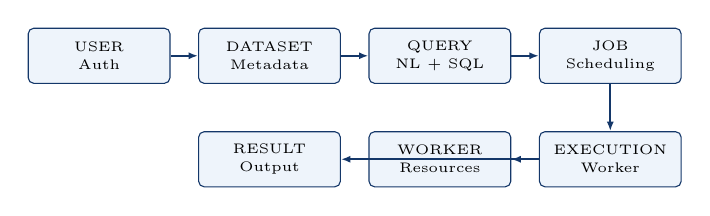
\begin{tikzpicture}[
node distance=3mm and 3.5mm,
entity/.style={
    rectangle,
    rounded corners=2pt,
    draw=GEUBlue,
    fill=GEULightBlue,
    minimum width=1.8cm,
    minimum height=7mm,
    align=center,
    font=\fontsize{5.5}{6.5}\selectfont
},
arrow/.style={
    -{Latex[length=1.2mm]},
    thick,
    draw=GEUBlue
}
]

\node[entity] (user) {USER\\Auth};
\node[entity,right=of user] (dataset) {DATASET\\Metadata};
\node[entity,right=of dataset] (query) {QUERY\\NL + SQL};
\node[entity,right=of query] (job) {JOB\\Scheduling};

\node[entity,below=6mm of job] (execution) {EXECUTION\\Worker};
\node[entity,left=of execution] (worker) {WORKER\\Resources};
\node[entity,left=of worker] (result) {RESULT\\Output};

\draw[arrow] (user) -- (dataset);
\draw[arrow] (dataset) -- (query);
\draw[arrow] (query) -- (job);
\draw[arrow] (job) -- (execution);
\draw[arrow] (execution) -- (worker);
\draw[arrow] (execution) -- (result);

\end{tikzpicture}
\end{center}

\vspace{1mm}

\begin{columns}[T,totalwidth=\textwidth]

\column{.48\textwidth}
\textbf{\color{GEUBlue}\small Core Entities}
\begin{itemize}\itemsep1pt
\item[\tiny$\bullet$] \scriptsize Users, Datasets \& Schema Mapping
\item[\tiny$\bullet$] \scriptsize Generated SQL, Jobs \& Execution Metrics
\end{itemize}

\column{.48\textwidth}
\textbf{\color{GEUBlue}\small Database Responsibilities}
\begin{itemize}\itemsep1pt
\item[\tiny$\bullet$] \scriptsize Transactional isolation \& Referential integrity
\item[\tiny$\bullet$] \scriptsize Persistent execution logging \& indexing
\end{itemize}

\end{columns}

\smallnote{Detailed ER Diagrams will be finalized during Phase II database architecture execution.}

\end{frame}


% ============================================================
% 13. INITIAL PROGRESS
% ============================================================

\begin{frame}{Initial Progress \& Team Contribution}

\begin{columns}[T,totalwidth=\textwidth]

\column{.42\textwidth}
\textbf{\color{GEUBlue}\small Phase-I Progress}
\begin{itemize}\itemsep1.5pt
\item[\tiny$\bullet$] \scriptsize Problem definition \& scope established
\item[\tiny$\bullet$] \scriptsize System architecture \& tech stack finalized
\item[\tiny$\bullet$] \scriptsize Mapping of OS algorithms to job queues
\item[\tiny$\bullet$] \scriptsize Initial PostgreSQL entity definitions
\end{itemize}

\column{.56\textwidth}
\textbf{\color{GEUBlue}\small Team Allocation}

\vspace{1mm}
\fontsize{6}{7.5}\selectfont
\begin{tabularx}{\textwidth}{@{}p{1.4cm}p{1.3cm}X@{}}
\toprule
\textbf{Member} & \textbf{Role} & \textbf{Responsibilities} \\
\midrule
Raghvander & Team Lead & Architecture, requirements analysis \& module integration \\
Tanishk & Backend & FastAPI development, REST endpoints \& API routes \\
Tushar & DB / Query & PostgreSQL schema, query parser \& validation logic \\
Soyam & AI / Systems & LLM prompts, OS scheduling algorithm \& worker logic \\
\bottomrule
\end{tabularx}

\end{columns}

\end{frame}


% ============================================================
% 14. ASSUMPTIONS & SCOPE
% ============================================================

\begin{frame}{Assumptions \& Initial Scope}

\begin{columns}[T,totalwidth=\textwidth]

\column{.48\textwidth}
\begin{block}{Assumptions}
\scriptsize
\begin{itemize}\itemsep1pt
\item Dataset input format consists of structured CSV files.
\item Primary database operations rely on PostgreSQL.
\item LLM API access remains available for query synthesis.
\item Workers operate in a bounded multi-process environment.
\end{itemize}
\end{block}

\column{.48\textwidth}
\begin{block}{Scope Boundaries}
\scriptsize
\begin{itemize}\itemsep1pt
\item Web dashboard for query entry \& visualization.
\item Natural-language-to-SQL translation layer.
\item SQL security filter preventing destructive statements.
\item OS-inspired CPU job scheduling algorithms.
\end{itemize}
\end{block}

\end{columns}

\vspace{2mm}

\begin{center}
\colorbox{GEULightBlue}{
\parbox{.88\textwidth}{
\centering\scriptsize
\textbf{Safety Protocol:} AI only assists query translation; query execution is strictly controlled by validation checks and OS scheduler rules.
}}
\end{center}

\end{frame}


% ============================================================
% 15. EXPECTED OUTCOMES
% ============================================================

\begin{frame}{Project Outcome / Deliverables}

\begin{columns}[T,totalwidth=\textwidth]

\column{.48\textwidth}
\textbf{\color{GEUBlue}\small Application Deliverables}
\begin{enumerate}\itemsep1.5pt
\scriptsize
\item Web portal for interactive data analysis
\item Role-based authentication system
\item Dataset parser \& automatic schema detector
\item Natural-language query translation module
\item SQL validation and safety guardrails
\end{enumerate}

\column{.48\textwidth}
\textbf{\color{GEUBlue}\small Systems Deliverables}
\begin{enumerate}\itemsep1.5pt
\scriptsize
\item Multi-algorithm job scheduler
\item Concurrent worker execution pool
\item Real-time resource usage monitoring
\item Query history \& execution log system
\item Comparative performance benchmark suite
\end{enumerate}

\end{columns}

\vspace{3mm}

\begin{center}
\colorbox{GEULightBlue}{
\parbox{.88\textwidth}{
\centering\scriptsize
The final software platform integrates \textbf{AI, DBMS, Operating Systems, and Distributed Systems} into a single functional analytical application.
}}
\end{center}

\end{frame}


% ============================================================
% 16. ROADMAP
% ============================================================

\begin{frame}{Development Roadmap}

\begin{center}
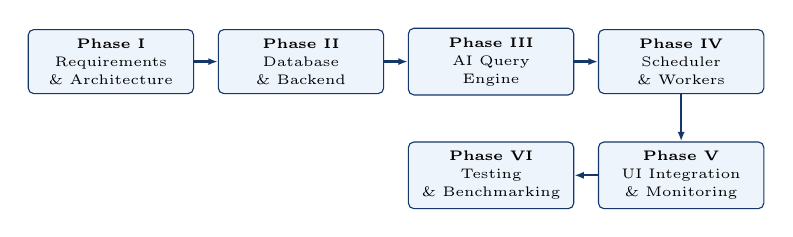
\begin{tikzpicture}[
phase/.style={
    rectangle,
    rounded corners=2pt,
    draw=GEUBlue,
    fill=GEULightBlue,
    minimum width=2.1cm,
    minimum height=8mm,
    align=center,
    font=\fontsize{5.5}{6.5}\selectfont
},
arrow/.style={
    -{Latex[length=1.2mm]},
    thick,
    draw=GEUBlue
}
]

\node[phase] (p1) {\textbf{Phase I}\\Requirements\\\& Architecture};
\node[phase,right=3mm of p1] (p2) {\textbf{Phase II}\\Database\\\& Backend};
\node[phase,right=3mm of p2] (p3) {\textbf{Phase III}\\AI Query\\Engine};
\node[phase,right=3mm of p3] (p4) {\textbf{Phase IV}\\Scheduler\\\& Workers};

\node[phase,below=6mm of p4] (p5) {\textbf{Phase V}\\UI Integration\\\& Monitoring};
\node[phase,left=3mm of p5] (p6) {\textbf{Phase VI}\\Testing\\\& Benchmarking};

\draw[arrow] (p1) -- (p2);
\draw[arrow] (p2) -- (p3);
\draw[arrow] (p3) -- (p4);
\draw[arrow] (p4) -- (p5);
\draw[arrow] (p5) -- (p6);

\end{tikzpicture}
\end{center}

\vspace{2mm}

\begin{columns}[T,totalwidth=\textwidth]

\column{.48\textwidth}
\textbf{\color{GEUBlue}\small Phase-I Focus (Current)}
\begin{itemize}\itemsep1pt
\item[\tiny$\bullet$] \scriptsize Domain definition, research gap analysis
\item[\tiny$\bullet$] \scriptsize Architectural pipeline \& database design
\end{itemize}

\column{.48\textwidth}
\textbf{\color{GEUBlue}\small Subsequent Focus}
\begin{itemize}\itemsep1pt
\item[\tiny$\bullet$] \scriptsize Core backend logic, scheduling engine
\item[\tiny$\bullet$] \scriptsize System evaluation \& benchmarking
\end{itemize}

\end{columns}

\end{frame}


% ============================================================
% 17. REFERENCES
% ============================================================

\begin{frame}{References}

\begin{enumerate}\itemsep3pt
\scriptsize
\item Sikha Bagui, Marta Malagutti, Riccardo Morelli, and Michael Tamascelli,
``Large Language Models in Database Management System Optimization: A Survey,''
\textit{ACM Transactions on Intelligent Systems and Technology}, Vol. 17, No. 5, 2026.
DOI: \href{https://doi.org/10.1145/3829078}{\texttt{10.1145/3829078}}

\item P. A. Prakash et al.,
``AI-Powered Transformer Framework for Intelligent Natural Language to SQL Query Generation,''
in \textit{Proc. Int. Conf. Smart Futuristic Technology (ICSFT)}, 2026.
DOI: \texttt{10.1109/ICSFT66733.2026.11507944}
\end{enumerate}

\vspace{2mm}

\begin{block}{Supporting Technical Documentation}
\scriptsize
\begin{itemize}\itemsep1pt
\item[\tiny$\bullet$] PostgreSQL, FastAPI, and Redis Official Technical Manuals
\item[\tiny$\bullet$] Operating Systems CPU Scheduling and Concurrency Literature
\end{itemize}
\end{block}

\end{frame}


% ============================================================
% 18. THANK YOU
% ============================================================

\begin{frame}[plain]

\begin{tikzpicture}[remember picture,overlay]

\draw[
    GEUBlue,
    line width=3pt
]
(current page.north west)
--
(current page.north east);

\node[
    anchor=north east,
    xshift=-0.45cm,
    yshift=-0.35cm
]
at (current page.north east)
{\IfFileExists{\GEULogo}{\includegraphics[height=0.9cm]{\GEULogo}}{\rule{0.9cm}{0.9cm}}};

\node[
    align=center,
    text width=.80\paperwidth
]
at (current page.center)
{

{\color{GEUBlue}
\fontsize{26}{30}\selectfont
\bfseries NEXUS}

\\[3mm]

{\color{GEUGrey}
\large
AI-Powered Distributed Data Processing\\
\& Compute Orchestration Platform}

\\[8mm]

{\color{GEUBlue}
\fontsize{18}{22}\selectfont
\bfseries Thank You}

\\[2mm]

\small Questions \& Suggestions

};

\node[
    align=center,
    anchor=south,
    yshift=.35cm
]
at (current page.south)
{
\small\bfseries
Department of Computer Science \& Engineering\\
Graphic Era (Deemed to be University), Dehradun
};

\end{tikzpicture}

\end{frame}

\end{document}